\renewcommand{\theequation}{\theenumi}
\renewcommand{\thefigure}{\theenumi}
\renewcommand{\thetable}{\theenumi}
\begin{enumerate}[label=\thesection.\arabic*.,ref=\thesection.\theenumi]
\numberwithin{equation}{enumi}
\numberwithin{figure}{enumi}
\numberwithin{table}{enumi}


\item Let U and V be two independent zero mean Gaussian random variables of variances $\dfrac{1}{4}$ and $\dfrac{1}{9}$ respectively. The probability $P(3V\geqslant2U)$ is
\begin{enumerate}
\begin{multicols}{4}
\setlength\itemsep{2em}
\item $
\dfrac{4}{9}
$
\item $
\dfrac{1}{2}
$
\item $
\dfrac{2}{3}
$
\item $
\dfrac{5}{9}
$
\end{multicols}
\end{enumerate}
%
\item Consider a binary digital communication system with equally likely 0's and 1's. When binary 0 is transmitted the voltage at the detector input can lie between the level -0.25V and +0.25V with equal probability: when binary 1 is transmitted, the voltage at the detector can have any value between 0 and 1V with equal probability. If the detector has a threshold of 2.0V (i.e., if the received signal is greater than 0.2V, the bit is taken as 1), the average bit error probability is
\begin{enumerate}
\begin{multicols}{4}
\setlength\itemsep{2em}

\item 0.15
\item 0.2
\item 0.05
\item 0.5
\end{multicols}
\end{enumerate}
%
\item Let X be the Gaussian random variable obtained by sampling the process at $t=t_i$ and let 
\begin{equation*}
Q(\alpha)={\int_{\alpha}^{\infty}}\dfrac{1}{\sqrt{2\pi}}e^{\frac{-y^2}{2}}dy
\end{equation*}
%
The probability that $[\textit{X}\leqslant1]$ is \dots
%
\item Let X be a zero mean unit variance Gaussian random variable. $E[|X|]$ is equal to .........
%
\\
\solution
Mean = $\mu$ = 0\\
Variance = $\sigma$ = 1\\
Gaussian Probability Distribution Function
\begin{align}
    &= f(x)\\
    &= \frac{1}{\sqrt{2\pi\sigma}} \exp{\left(\frac{-(x - \mu)^2}{2\sigma^2}\right)}\\
    &= \frac{1}{\sqrt{2\pi}} \exp{ \left(\frac{-x^2}{2}\right)}
\end{align}
\begin{align}
    \mean{ \abs X} &= \int _{-\infty} ^{\infty} \abs x f(x)\\
    &= 2 \int _{0} ^{\infty} x f(x) dx \\
    &= 2 \int _{0} ^{\infty} x \frac{1}{\sqrt{2\pi}}  \exp{\left(\frac{-x^2}{2}\right)} dx\\
    &= \sqrt{\frac{2}{\pi}} \int _{0} ^{\infty} x  \exp {\left(\frac{-x^2}{2}\right)} dx\\
    &= \sqrt{\frac{2}{\pi}} \int _{0} ^{\infty} (-1) \exp{(u)} du
\end{align}
(Using substitution)\\
\begin{align}
    &= \sqrt{\frac{2}{\pi}}\\
    &= 0.7978
\end{align}

\item Consider a discrete-time channel $Y = X+Z$, where the additive noise Z is signal-dependent. In particular, given the transmitted symbol $X \in \{-a,+a\}$ at any instant, the noise sample Z is chosen independently from a Gaussian distribution with mean $\beta X$ and unit variance. Assume a threshold detector with zero threshold at the receiver.\\
When $\beta = 0$, the BER was found to be $Q(a) = 1 \times {10^-8}$.\\
$$
\bigg(Q(v)= \dfrac{1}{\sqrt{2 \pi}} \int_{v}^{\infty} e^{\frac{-u^2}{2}}du$$, and for $v>1$, use $Q(v) \approx e^{\frac{-v^2}{2}} \bigg)$ \\
When $\beta = -0.3$, the BER is closet to

\begin{enumerate}
\begin{multicols}{2}
\setlength\itemsep{2em}

\item $10^-7$
\item $10^-6$
\item $10^-4$ \label{option C}
\item $10^-2$

\end{multicols}
\end{enumerate}
%
\solution

Given that the threshold of the detector is zero. Define a detector function $g$ such that
\begin{align}
g(Y) = 
\begin{cases}
+a & Y>0 \\
-a & Y<0
\end{cases}
\end{align}
It is given that $X \in \{ -a, a\}$ is a random variable.
\begin{align}
\therefore \Pr(X=a) = \Pr(X=-a) = \dfrac{1}{2}
\end{align}
Since the noise in the signal, $Z$ is chosen independently from a Gaussian distribution with mean $ \mu = \beta X$ and unit variance, it follows that
\begin{align}
F_Z(z) &= \int_{-\infty}^{z} \dfrac{1}{\sqrt{2\pi}} \exp \left( \dfrac{-(z - \beta X)^2}{2} \right) dz \\
&= \int_{-\infty}^{z - \beta X} \dfrac{1}{\sqrt{2\pi}} \exp \left( \dfrac{-z^2}{2} \right) dz \\
&= \int_{\beta X-z}^{\infty} \dfrac{1}{\sqrt{2\pi}} \exp \left( \dfrac{-z^2}{2} \right) dz \\
&= Q(\beta X - z) \label{eqn 2.0.7}
\end{align}
Also, it is easy to see that 
\begin{align}
Q(-v) = 1 - Q(v) \; \forall \; v \in \mathbb{R} \label{eqn 2.0.8}
\end{align}
The detector can record erroneous bits in the signal iff
\begin{align}
X>0 \; &, \; g(Y) = -a \; (\text{Call this BER}_{+a}) \text{ or}\\
X<0 \; &, \; g(Y) = a \; (\text{Call this BER}_{-a})
\end{align}
\begin{align}
\therefore \text{BER}_{+a} % &= \Pr(g(Y) = -a \;,\; X = a)\\
&= \Pr(g(Y) = -a \;|\; X = a) \Pr(X=a)\\
&= \Pr(Y < 0 \;|\; X = a) \Pr(X=a)\\
&= \dfrac{1}{2} \times \Pr(X+Z < 0 \;|\; X = a) \\
% &= \dfrac{1}{2} \times \Pr(a+Z < 0 \;|\; X = a) \\
% &= \dfrac{1}{2} \times \Pr(Z < -a \;|\; X = a) \\
&= \dfrac{1}{2} \times F_Z(-a)\\
&= \dfrac{1}{2} \times Q(\beta X + a) \; \text{ (From (\ref{eqn 2.0.7}))}\\
% &= \dfrac{1}{2} \times Q(a \beta + a)\\
&= \dfrac{1}{2} \times Q(a(1+\beta))
\end{align}
\begin{align}
\text{BER}_{-a} % &= \Pr(g(Y) = a \;,\; X = -a)\\
&= \Pr(g(Y) = a \;|\; X = -a) \Pr(X=-a)\\
&= \Pr(Y > 0 \;|\; X = -a) \Pr(X=-a)\\
&= \dfrac{1}{2} \times \Pr(X+Z > 0 \;|\; X = -a) \\
% &= \dfrac{1}{2} \times \Pr(Z-a > 0 \;|\; X = -a) \\
% &= \dfrac{1}{2} \times \Pr(Z > a \;|\; X = -a) \\
&= \dfrac{1}{2} \times \left( 1 - F_Z(a) \right) \\
&= \dfrac{1}{2} \times \left( 1 - Q(\beta X -a) \right) \; \text{ (From (\ref{eqn 2.0.7}))}\\
% &= \dfrac{1}{2} \times \left( 1 - Q(-a \beta -a) \right) \\
&= \dfrac{1}{2} \times Q(a(1+\beta)) \; \text{ (From (\ref{eqn 2.0.8}))}
\end{align}
\begin{align}
\therefore \text{BER} &= \text{BER}_{+a} + \text{BER}_{-a}\\
&= Q(a(1+\beta))
\end{align} 
\begin{figure}[!hbt]
    \centering
	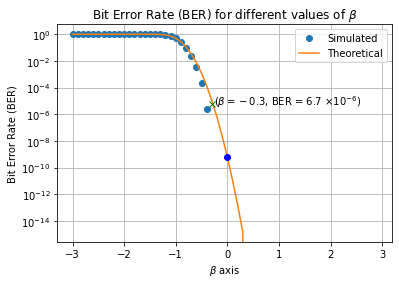
\includegraphics[width=\columnwidth]{solutions/ec/45/Figures/Figure_3.png}
    \caption{Theory vs Simulated plot of BER}
    \label{CDF_Y}
\end{figure}
When $\beta = 0$, it is given that 
\begin{align}
\text{BER} = Q(a) &= 10^{-8}
\end{align}
On computing, $Q(1) \approx 0.16$. Since $Q(a)<Q(1)$, it is easy to see that $a>1$ (as $Q(x)$ is a decreasing function)
\begin{align}
\therefore e^{-a^2 / 2} &= 10^{-8}\\
\Leftrightarrow a &\approx 6.069
\end{align}
When $\beta = -0.3$,
\begin{align}
\text{BER} = Q(a(1+\beta)) &= Q(6.069 \times (1-0.3))\\
&= Q(6.069 \times 0.7)\\
&= Q(4.249)\\
&\approx \exp (-\dfrac{4.249^2}{2})\\
&\approx 1.2 \times 10^{-4}
\end{align}
Therefore, when $\beta = -0.3$, BER is closest to $10^{-4}$ and option \ref{option C} is correct.


\item Suppose $X$ and $Y$ are two random variables such that $aX + bY$ is a normal random variable for all $a,b \in \mathbb{R}$. Consider the following statements P,Q,R and S:


 (P): $X$ is a standard normal random variable.\\
 (Q): The conditional distribution of $X$ given $Y$ is normal.\\
 (R): The conditional distribution of $X$ given $X$ + $Y$ is normal.\\
 (S): $X$ - $Y$ has mean $0$.\\

Which of the above statements ALWAYS hold TRUE?
\begin{enumerate}
\begin{multicols}{2}
\setlength\itemsep{2em}

\item both P and Q
\item both Q and R
\item both Q and S
\item both P and S

\end{multicols}
\end{enumerate}

\item A random variable $X$ takes values -1 and +1 with probabilities 0.2 and 0.8, respectively.
It is transmitted across a channel which adds noise $N$, so that the random variable at the
channel output is $Y = X + N$. The noise $N$ is independent of $X$, and is uniformly
distributed over the interval [-2 , 2]. The receiver makes a decision
\[
\hat{X} = \begin{cases}
            -1, &\text{if}\quad Y \leq \theta \\
             +1, &\text{if}\quad Y \geq \theta\\
            \end{cases}
\]
where the threshold $\theta  \in [-1,1]$ is chosen so as to minimize the probability of error
\pr {\hat{X} \neq X}. The minimum probability of error, rounded off to 1 decimal place, is \dots
\\
\solution

We know that 
\begin{align}
    X \in \{-1,+1\}\\
    N \in [-2,2]\\
    Y = X + N\\
    \pr{X = -1} = 0.2\\
    \pr{X = +1} = 0.8
\end{align}
Since $N$ is uniformly distributed\\
$\therefore$ the probability distribution function of $N$ is:

\begin{tikzpicture}[
  declare function={
    func(\x)= (\x < -2) * (0)   +
              and(\x >= -2, \x < 2) * (0.25)     +
              (\x >= 2) * (0)
   ;
  }
]
\begin{axis}[
  axis x line=middle, axis y line=middle,
  ymin=0, ymax=1, ytick={0,0.25,0.5,0.75,1}, ylabel=$f(N)$,
  xmin=-3, xmax=3, xtick={-3,...,3}, xlabel=$N$,
  domain=-3:3,
  samples=100,
]

\addplot [blue,thick] {func(x)};
\end{axis}
\end{tikzpicture}
\\
The cdf of this uniform probability distribution function is
\begin{align}
    F_X(x) &= \int_{-\infty}^xf(N)dN \\ 
    &=\int_{-2}^x\frac{1}{4}dN\\
    &=\frac{x+2}{4}\label{eq:0.0.8}
\end{align}
For $X \neq \hat{X}$ we need to check for each case. Using equation \eqref{eq:0.0.8}
\begin{align}
\therefore
    \pr{N>\theta + 1} &= 1-\pr{N < \theta + 1}\\
    &= 1-F_X(\theta + 1)\\
    &= 1- \frac{\theta + 3}{4}\\
    &= \frac{1}{4}(1-\theta)\label{eq:0.0.12}
\end{align}
\begin{align}
\therefore
    \pr{N < \theta-1} &= F_X(\theta - 1)\\
    &= \frac{1}{4}(1+\theta)\label{eq:0.0.14}
\end{align}
The probability of error:
\begin{align}
\nonumber
    \pr {\hat{X} \neq X} = P(-1)\cdot {P(\theta < -1 + N)} \\ 
            \quad+ P(1)\cdot {P(\theta> N + 1)}\label{eq:0.0.15}
\end{align}
Substituting \eqref{eq:0.0.12} and \eqref{eq:0.0.14} in \eqref{eq:0.0.15}. We get:
\begin{align}
\nonumber
    \pr {\hat{X} \neq X} &= 0.2\cdot \frac{1}{4}(1-\theta) \\
    & \quad+ 0.8\cdot \frac{1}{4}(1+\theta)
\end{align}
On simplifying the equation we get
\begin{align}
    \pr {\hat{X} \neq X} = \frac{1}{4} + \frac{3}{20}\theta
\end{align}
Since this is a linear equation in $\theta$, the minimum will occur at boundary points.
Putting $\theta = +1$, we get
\begin{align}
    \pr {\hat{X} \neq X} = 0.4
\end{align}
but on putting $\theta = -1$, we get
\begin{align}
    \pr {\hat{X} \neq X} = 0.1
\end{align}
Hence the value of probability of error is:
\begin{align}
    \therefore \pr {\hat{X} \neq X} = 0.1
\end{align}



%
\item  Let $U$ and $V$ be two independent zero mean Gaussian random variables of variances $\frac{1}{4}$ and $\frac{1}{9}$ respectively. The probability $\pr{3V\geq2U }$ is
\begin{enumerate}
    \item $4/9$
    \item $1/2$
    \item $2/3$
    \item $5/9$
\end{enumerate}
%
\solution

$U$ and $V$ are independent random variables,
For $V$, $\mu_V=0$, and $\sigma_V^2=\frac{1}{9}$
\begin{align}
    V\sim N\brak{0,\frac{1}{9}}
\end{align}
For $U$, $\mu_U=0$, and $\sigma_U^2=\frac{1}{4}$
\begin{align}
    U\sim N\brak{0,\frac{1}{4}}
\end{align}
Let,
\begin{align}
    Z=3V-2U\\
    Z\sim N\brak{\brak{3\mu_V-2\mu_U}, \brak{(3)^2\sigma_U^2+(2)^2\sigma_V^2}}\\
    Z\sim N\brak{0,9\times\frac{1}{9}+4\times\frac{1}{4}}\\
    Z\sim N\brak{0,2}
\end{align}
For $Z$, $\mu=0$, and $\sigma^2=2$.
By Gaussian Distribution,
Let $X$ is standard normal variable,
\begin{align}
    X=\frac{Z-\mu}{\sigma}\\
    \pr{Z\geq0}=\pr{X\sigma+\mu\geq0}\\
    \pr{Z\geq0}=\pr{X\brak{\sqrt{2}}+0\geq0}\\
    \pr{Z\geq0}=\pr{X\geq0}\\
    \pr{Z\geq0}=Q\brak{0}
\end{align}
where $Q(x)$ is the $Q-function$,
\begin{align}
    Q\brak{0}=\frac{1}{2}\\
    \pr{Z\geq0}=\frac{1}{2}\\
    \pr{3V-2U\geq0}=\frac{1}{2}\\
    \pr{3V\geq2U}=\frac{1}{2}
\end{align}
Option (B) is correct.
%


\end{enumerate}